\section{Metropolis Evaluation}
\counterwithin{figure}{section} %reset figure numbering

The metropolis algorithm was evaluated for 120,000 iterations, with the first 20,000 discarded as "burnin" iterations, during which the model was experiencing transient behavior. Our method is based on a markov chain, such that the proposed parameter values for each iteration were based on the values from the last accepted iteration according to:

\begin{equation}\label{eqn:proposal}
\begin{split}
delta&=Range(Prior) \\
Proposal_i&=Accepted_{i-1} + dp \cdot (0.5-rand) \cdot delta;
\end{split}
\end{equation}
where $delta$ is the range allowed by the uniform prior for each parameter and $rand$ is a random number between 0 and 1. $Proposal_i$ is the value of a parameter for iteration $i$ and $Accepted_{i-1}$ is the last value of that parameter accepted by the algorithm. To more efficiently explore parameter space, proposed parameters were selected with step sizes $dp_{Age}$ = 0.2 and $dp_{TWTT}$ = 0.1 for those parameters associated with each likelihood in Equation~\ref{eqn:bigproblem}.

The evaluation of the two likelihood functions, or cost, are independently accepted according to each function's metropolis probability during each iteration. The accepted cost solutions for each cost, depth and age, are shown in Figure~\ref{fig:cost}. As seen in the figure, these cost values show little trend aside from occasional positive departures from the mean as the model explores parameter space. 

\begin{figure*}[ht]
%\begin{center}
\centering
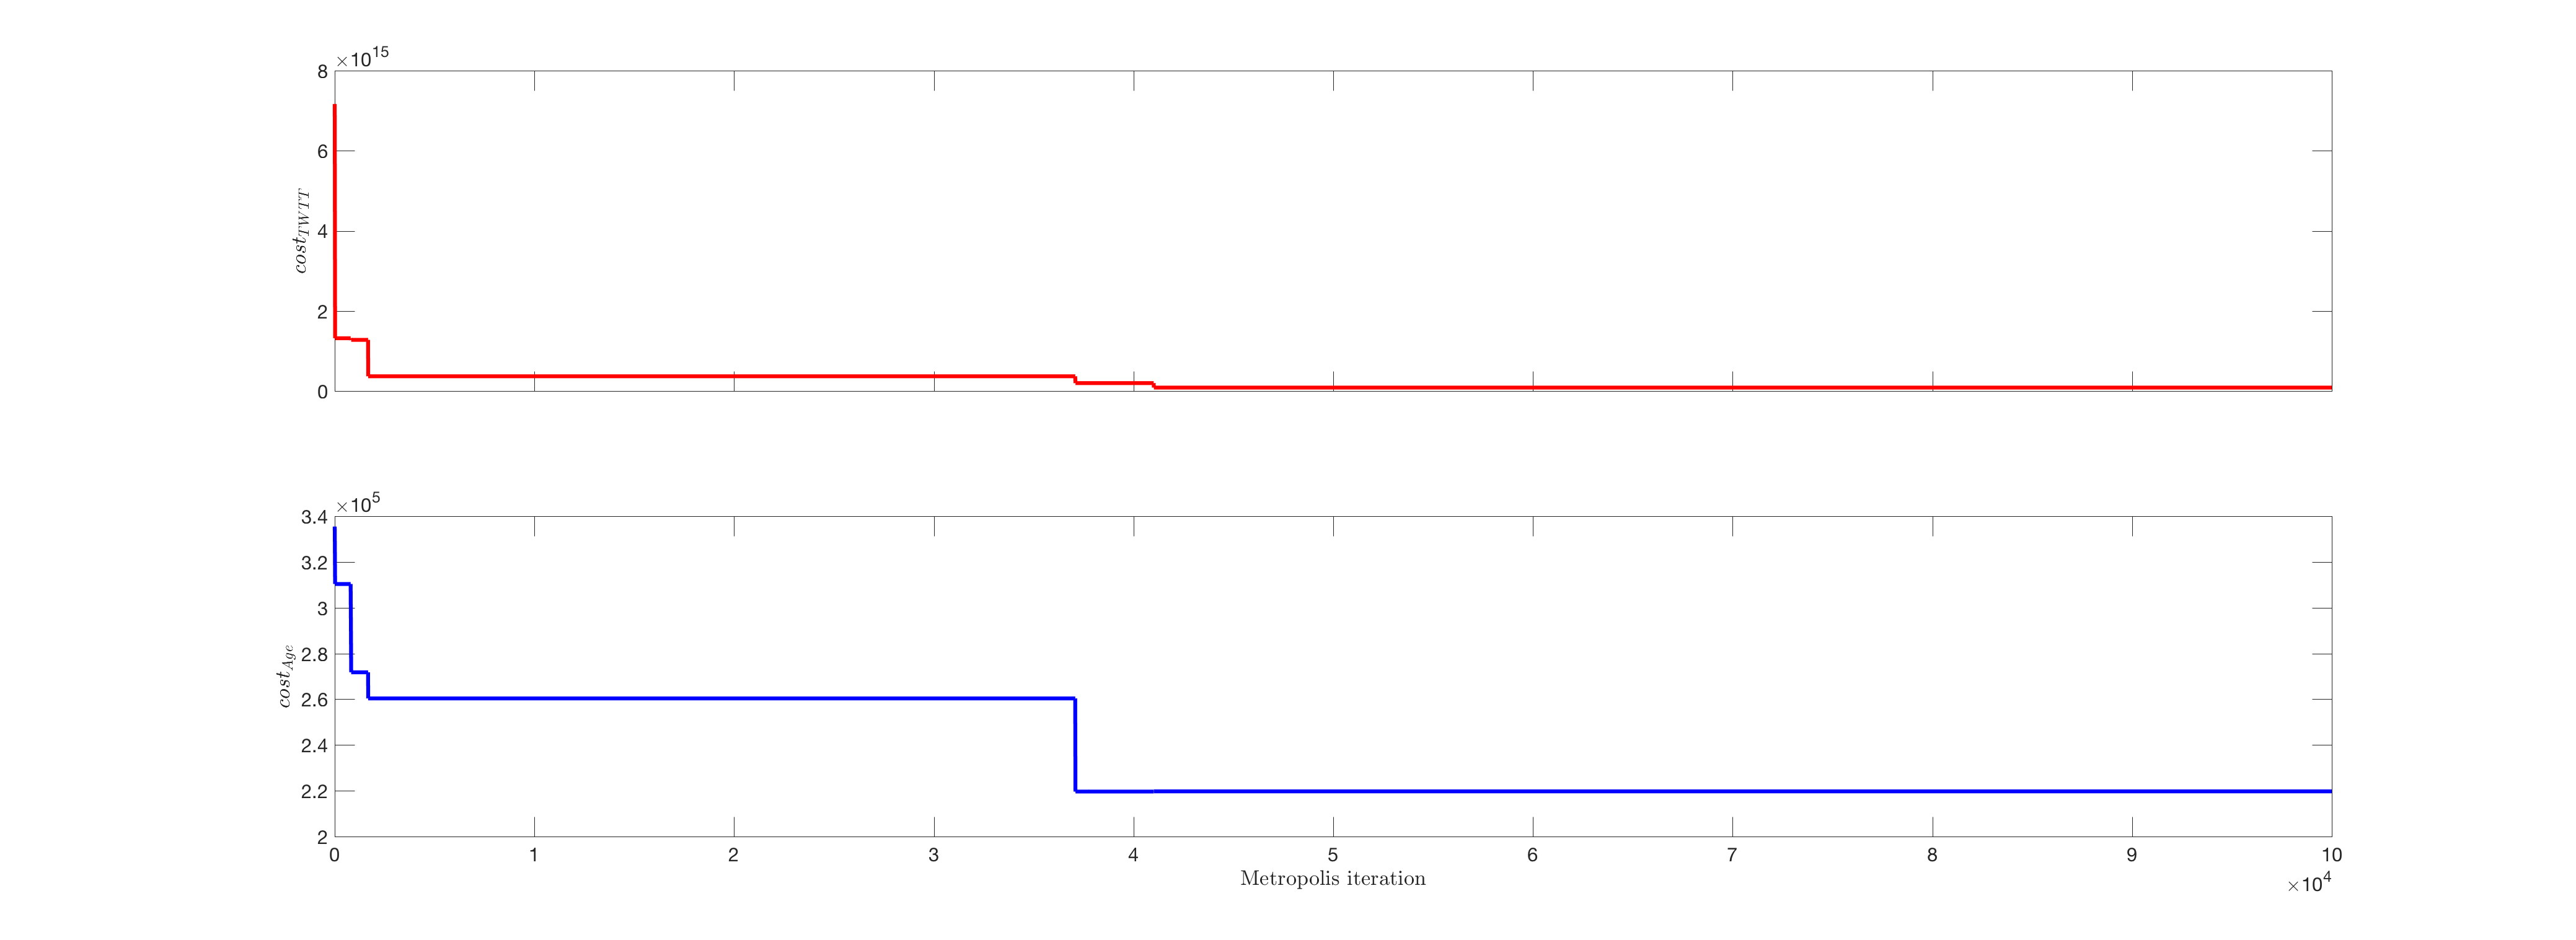
\includegraphics[scale=0.3]{../analysis/figures/cost}
%\captionsetup{width=.9\textwidth}
\caption[]{Cost of the age and depth likelihood functions at each accepted iteration.}
%\end{center}
\label{fig:cost}
\end{figure*}





\section{Degrees of freedom and parameter correlation}
\counterwithin{figure}{section} %reset figure numbering

As we invert for model parameter values, we anticipate the data points used to constrain our likelihood functions -- sourced from radar observations and Byrd ice core volcanic chronology -- are not independent of one another. As a result, we expect the number of degrees of freedom to be less than the number of data points available. While we do not know the exact number of effective degrees of freedom, $k_e$, we explore the sensitivity of our results to our choice of $k_e$ (Figure~\ref{fig:ke}). We find that our choice does not significantly impact the mean estimates of age or depth for our radar reflectors. Conservatively, we choose to assume $k_e$ = N$_{data}$/4 = 15.25 because the uncertainties are largest while not changing the mean estimates. 

\begin{figure*}[ht]
%\begin{center}
\centering
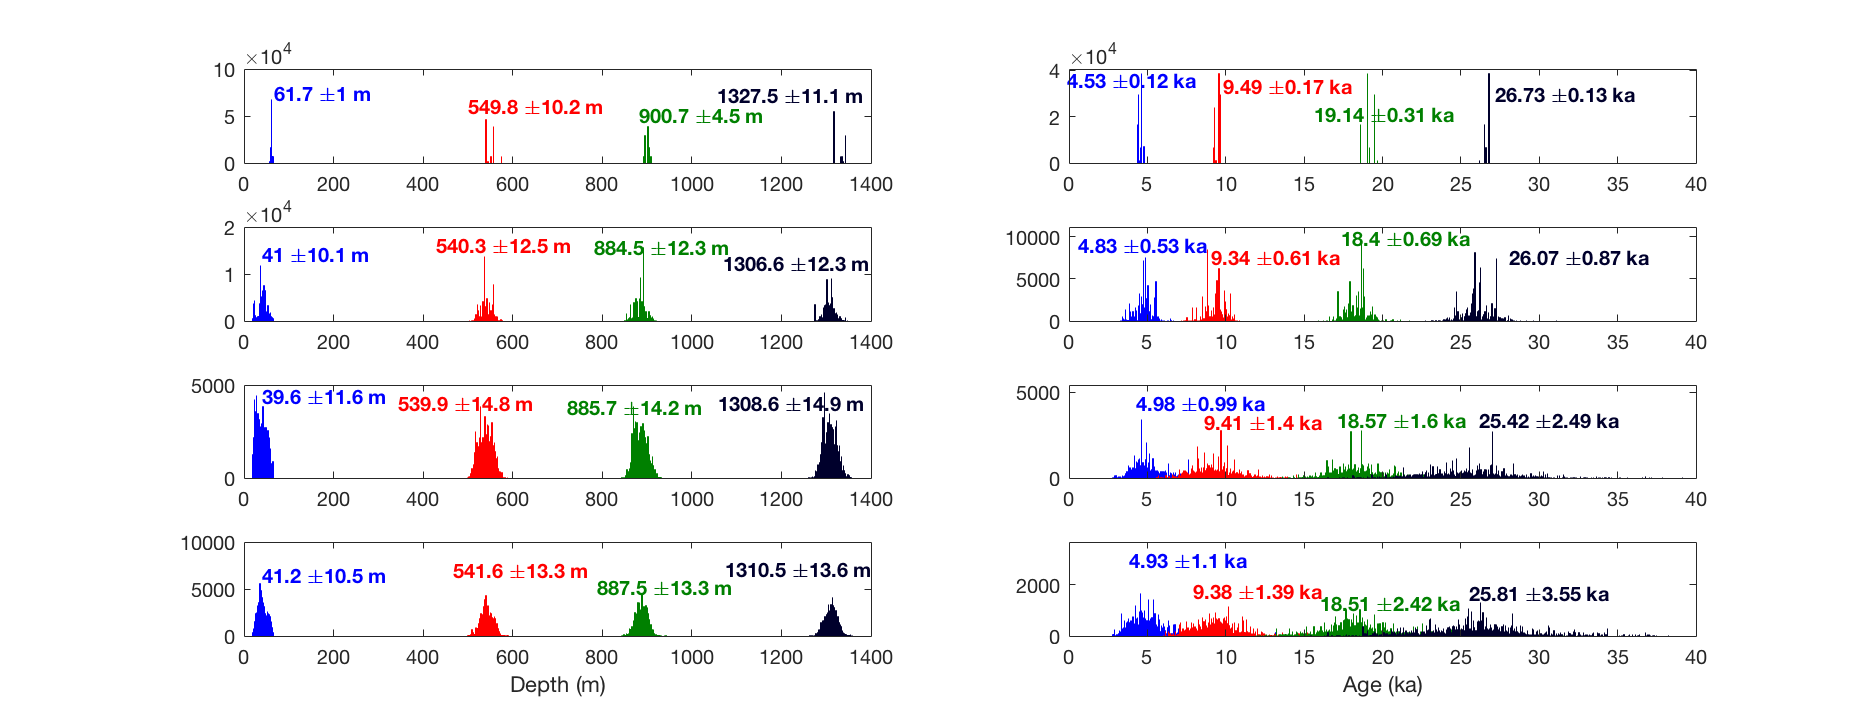
\includegraphics[scale=0.3]{../analysis/figures/keCompare_tweaked}
%\captionsetup{width=.9\textwidth}
\caption[]{Comparison of results for reflector age and depth assuming a range of $k_e$ values. All agree to within uncertainty.}
%\end{center}
\label{fig:ke}
\end{figure*}

Figure~\ref{fig:flowparamconvergence} shows the results of inverting for several model parameters in this problem, including flow parameters such as $q$ as well as ice property parameters such as $v_{ice}$. The results show the parameters are not correlated with one another and do seem to convergence to most-likely solutions.

\begin{figure*}[ht]
%\begin{center}
\centering
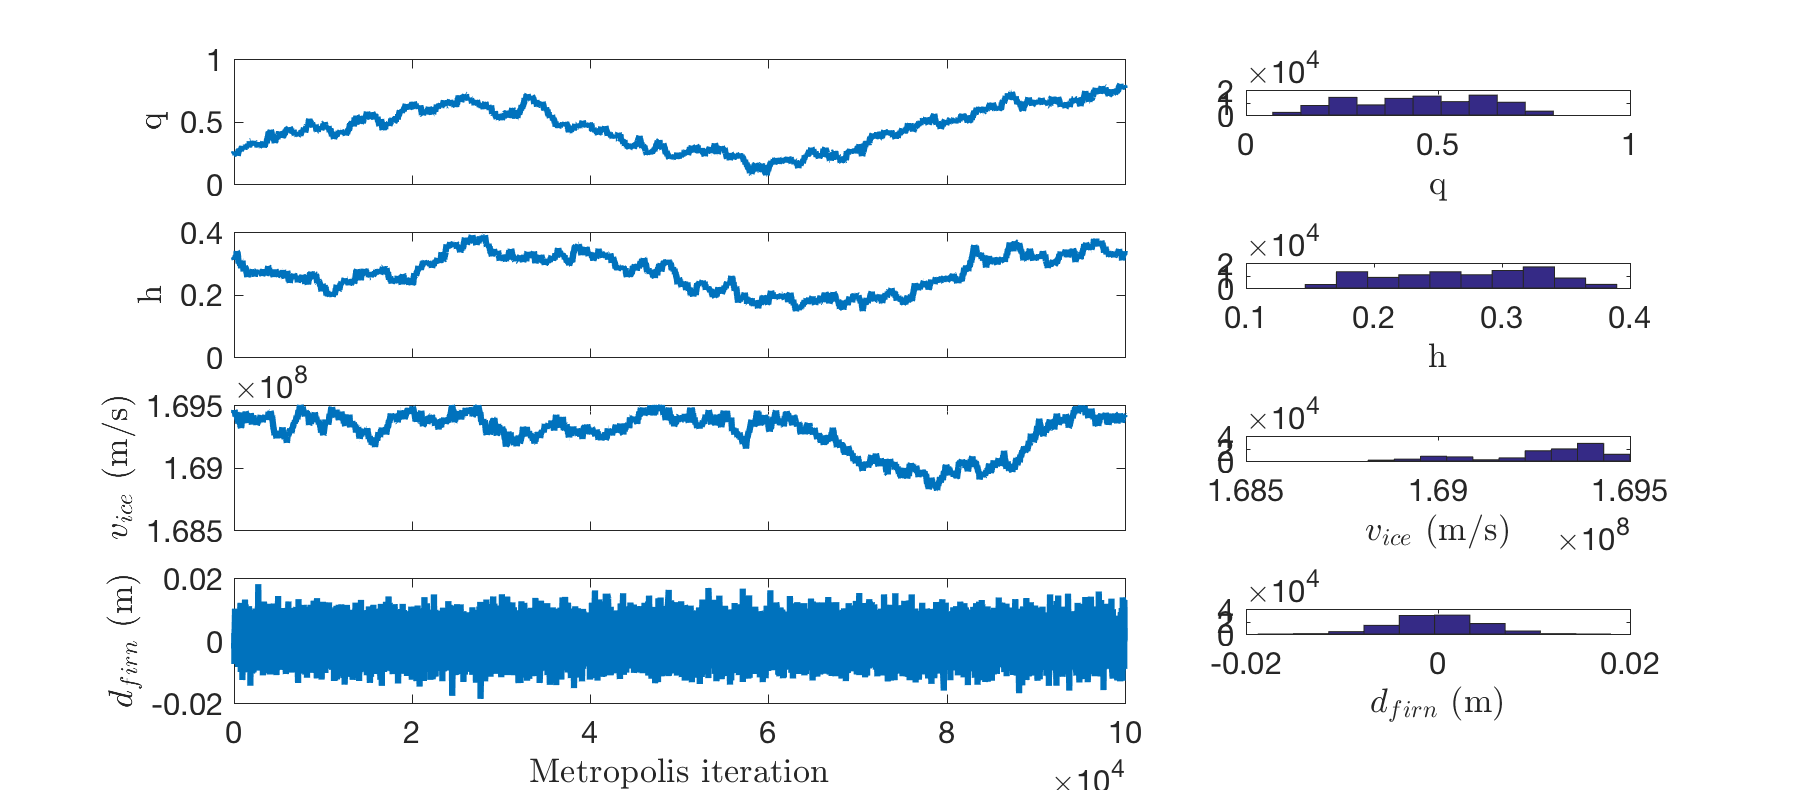
\includegraphics[scale=0.3]{../analysis/figures/convergence1}
%\captionsetup{width=.9\textwidth}
\caption[]{Left: Flow parameter values at each accepted Metropolis iteration for parameters $q$ (top), $h$, $v_{ice}$, and $d_{firn}$ (bottom). The parameter values do not appear correlated Right: Histograms of the parameter values shown in the left column. Histograms show the parameter values converging.}
%\end{center}
\label{fig:flowparamconvergence}
\end{figure*}

Accumulation rate is divided into 10 parameters, each covering a depth bin of $\sim$200 m. This allows for variation in the accumulation rate over time, as expected. The resulting accumulation rate profiles are shown in Figure~\ref{fig:accumdepth}. As discussed previously and further in Section~\ref{sec:regularization}, these profiles have been regularized to select profiles which do not exhibit an unrealistic amount of variability. In Figure~\ref{fig:accumdepth}, they have been additionally sorted by cost to demonstrate the relative quality of the accepted solutions.

\begin{figure*}[ht]
%\begin{center}
\centering
\includegraphics[scale=0.3]{../analysis/figures/accumdepthSorted}
%\captionsetup{width=.9\textwidth}
\caption[]{Accumulation rate as a function of ice depth colored by cost value for the estimated parameter values. (Accumulation rate series associated with lower cost are expected to be solutions.) Accumulation rate is estimated in 10 depth bins at $\sim$200 m depth intervals. Transitions between these intervals have been smoothed in this figure for each of viewing.}
%\end{center}
\label{fig:accumdepth}
\end{figure*}

To further explore the accumulation rate solutions, we look at the accepted parameter values and their convergence over all iterations. As seen in the right side of Figure~\ref{fig:accumconvergence}, the accumulation rate solutions do not converge as readily as other parameters, leaving wider distributions exhibiting more uncertainty in our estimates of accumulation rate. This may mean that our priors play an important role in estimating the value of accumulation rate and therefore the result could be improved with a more informative prior. 

We see correlation between some accumulation rate parameters (left side of Figure~\ref{fig:accumconvergence}). This may indicate we could have combined these accumulation rate depth bins and/or that additional iterations may be useful. Figure~\ref{fig:accumCorrelation} shows a correlation matrix between each accumulation rate parameter and every other. Along the diagonal are histograms of each accumulation rate parameter. Those parameter pairs with correlation coefficients greater than 0.5 are shown in yellow. Highly correlated pairs of accumulation rate parameters tend to occur in the middle of the ice column between 600 m and 1400 m depth. \textbf{(Any idea why?)}

\begin{figure*}[ht]
%\begin{center}
\centering
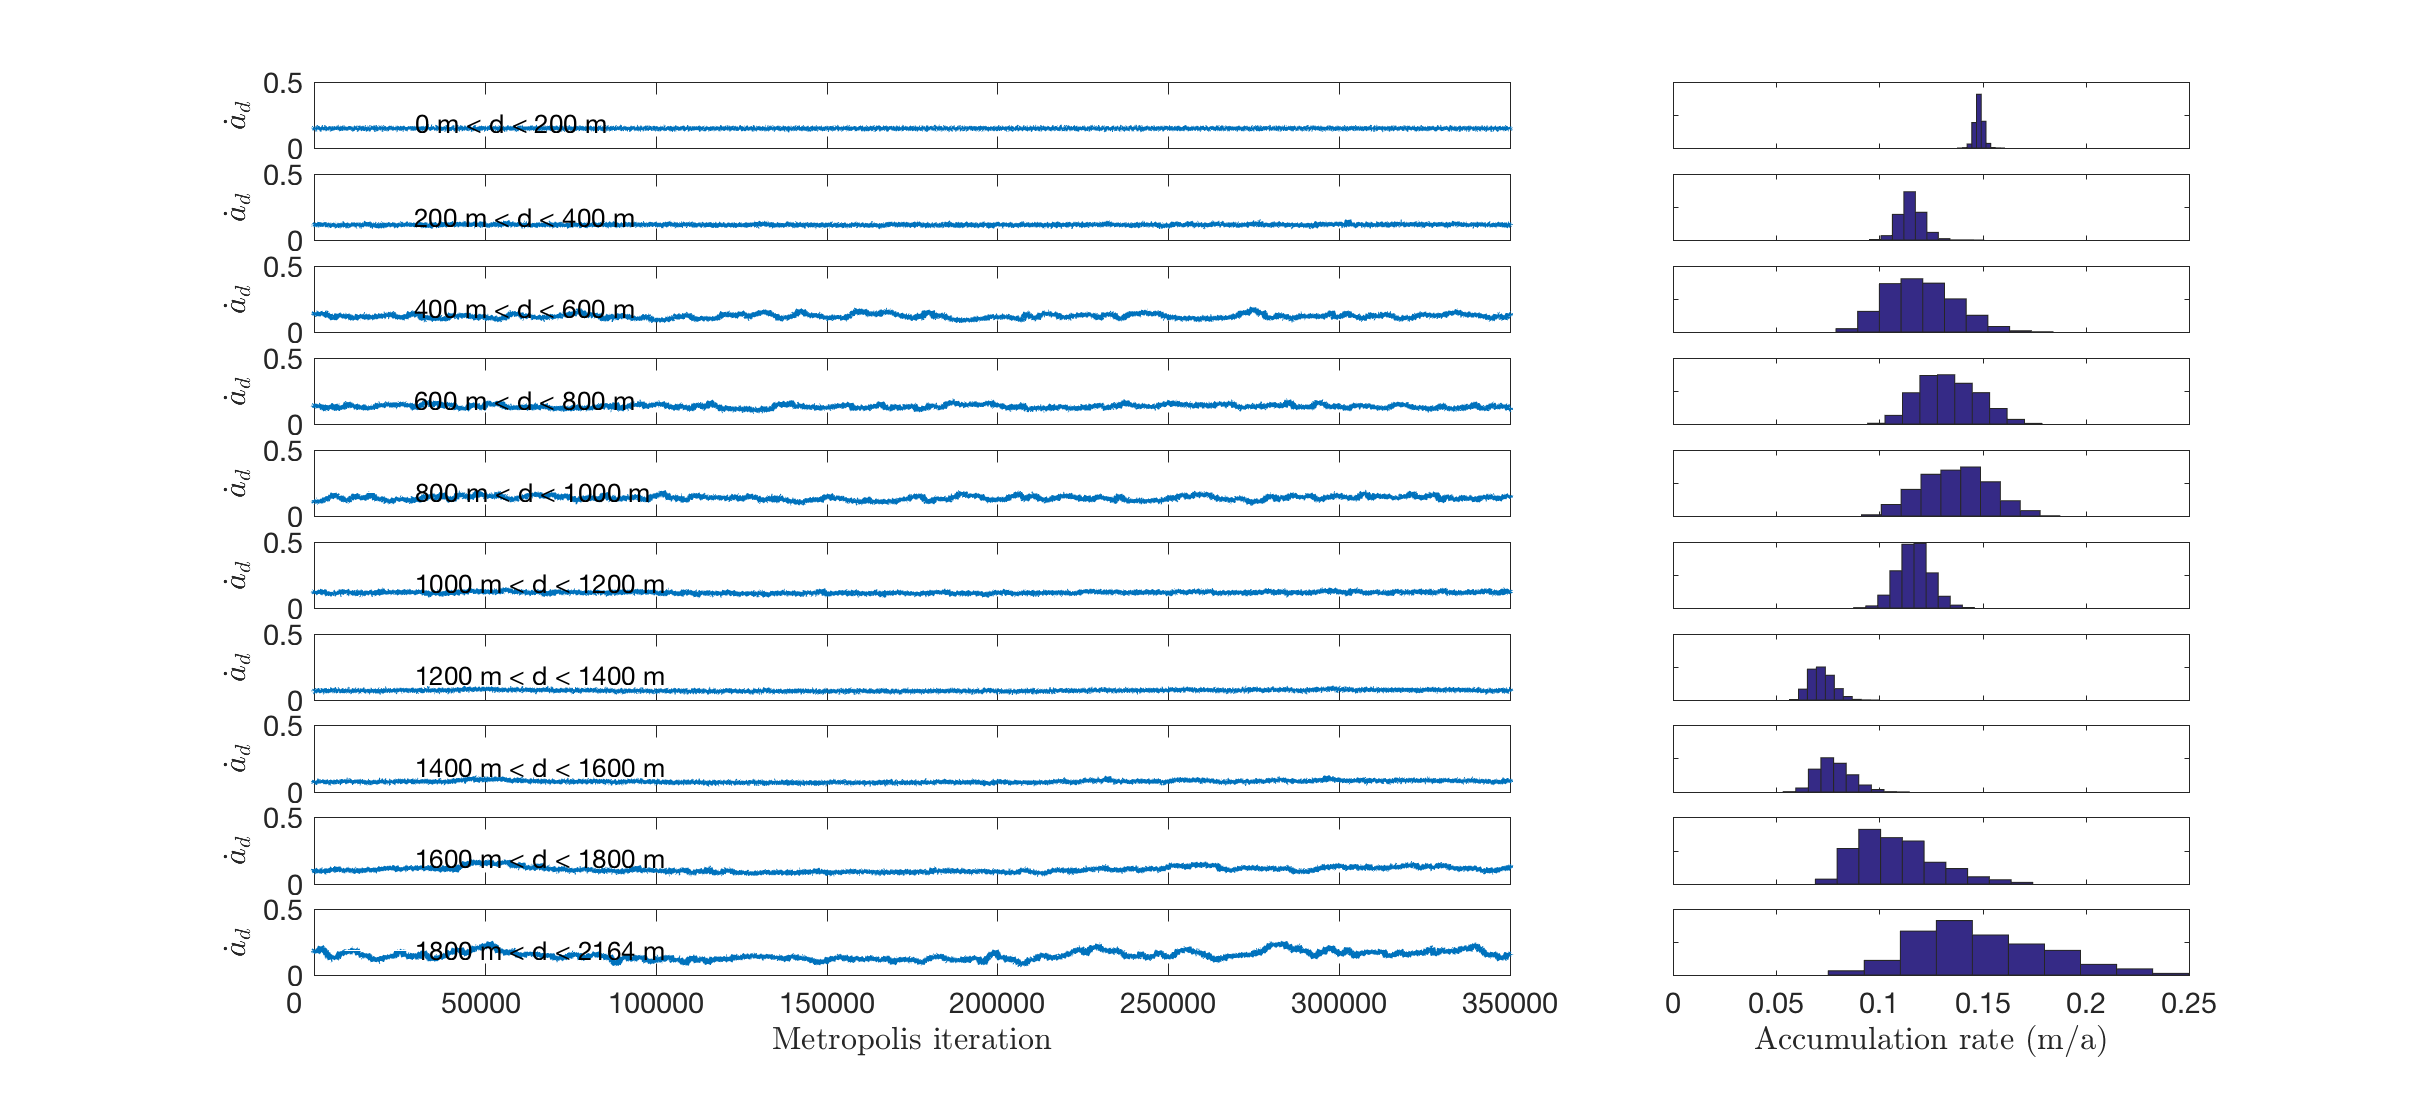
\includegraphics[scale=0.3]{../analysis/figures/convergence2}
%\captionsetup{width=.9\textwidth}
\caption[]{Left: Values of each accumulate rate parameter (in each of 10 depth bins, shallowest at top). Right: Histograms of the parameter values at left. Certain depth bins appear to be correlated and the histograms of values are wider, indicating the accumulation rate parameters are slower to converge and more uncertain.}
%\end{center}
\label{fig:accumconvergence}
\end{figure*}

\begin{figure*}[ht]
%\begin{center}
\centering
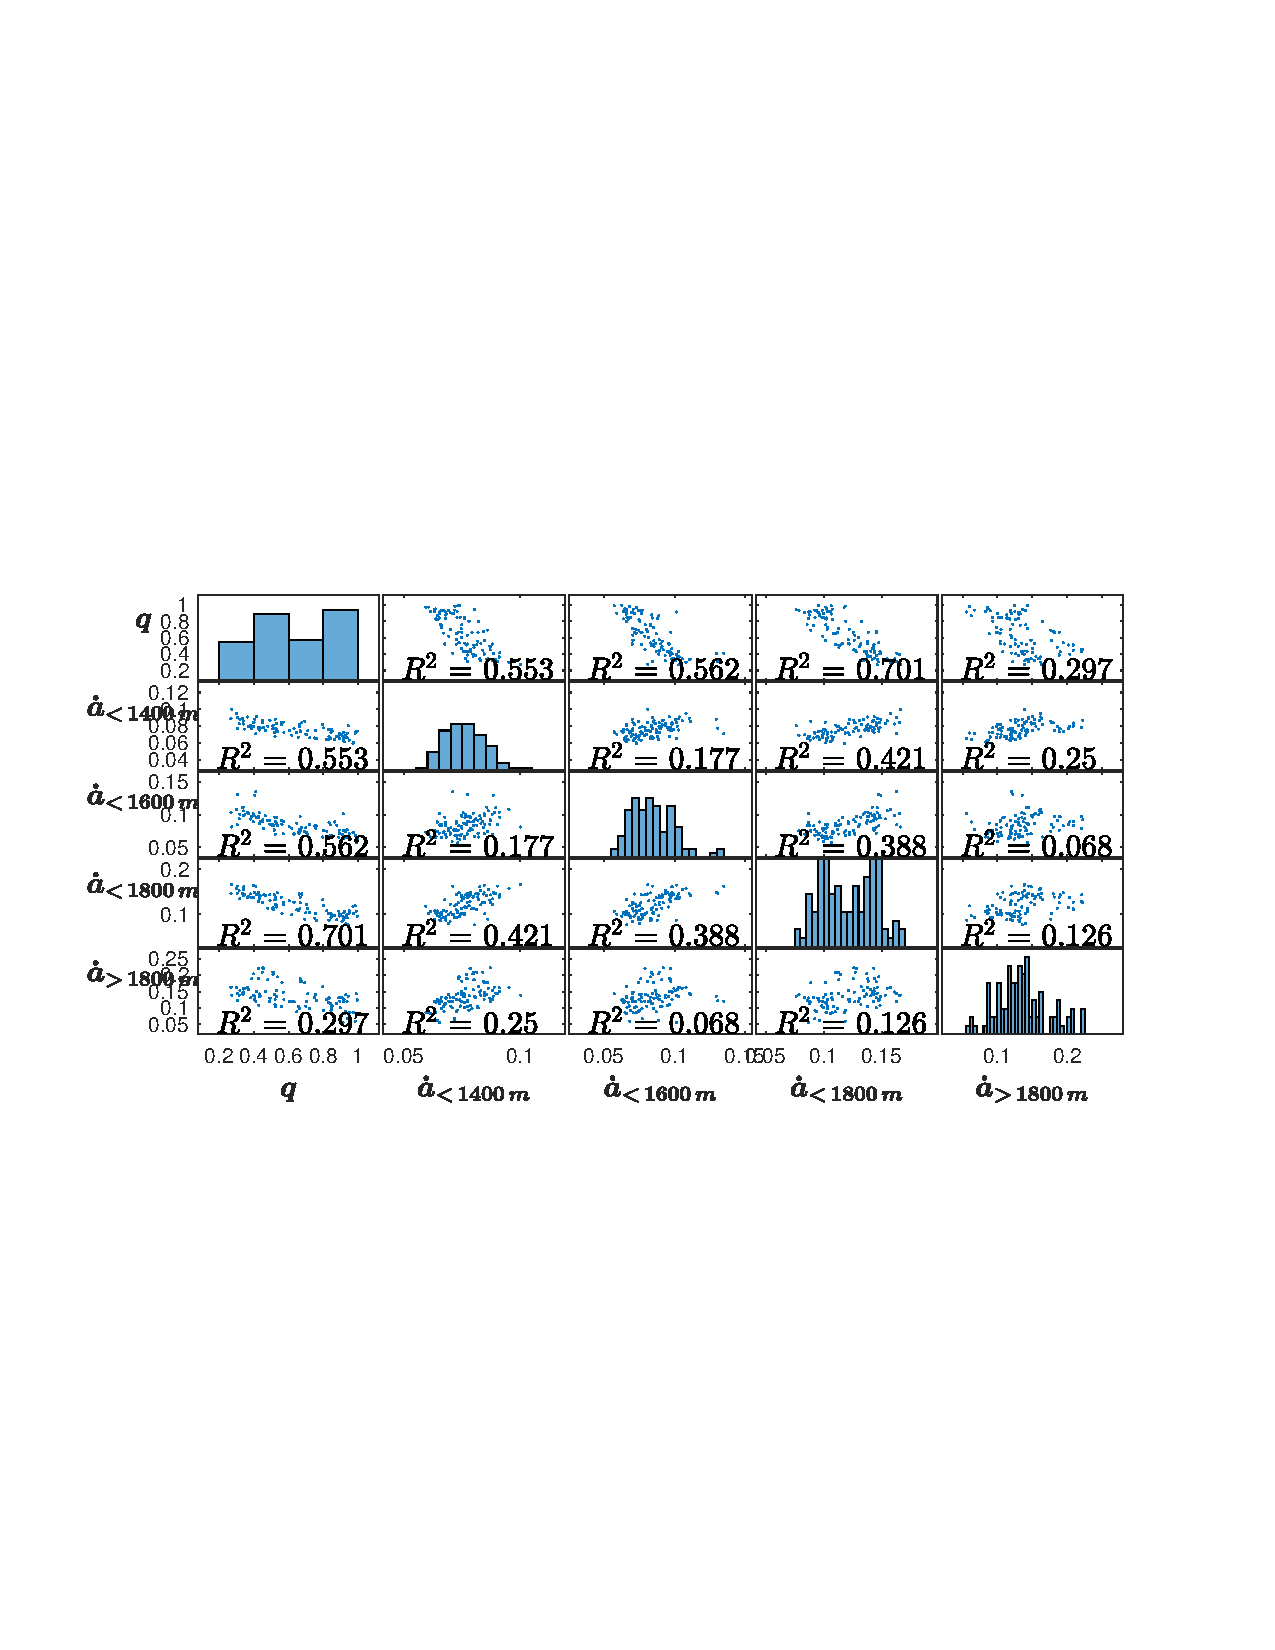
\includegraphics[scale=0.3]{../analysis/figures/accumCorrelation}
%\captionsetup{width=.9\textwidth}
\caption[]{Correlation of each accumulation rate parameter with every other accumulation rate parameter. Histograms of each accumulation rate are shown along the diagonal. Yellow plots indicate pairs of parameters with correlation coefficients above 0.5. Correlation is gneerally highest between accumulation rate parameters in the middle of the ice column, between 600 and 1400 m depth.}
%\end{center}
\label{fig:accumCorrelation}
\end{figure*}


Convergence of the reflector depths is shown in Figure~\ref{fig:depthconvergence}.


\begin{figure*}[ht]
%\begin{center}
\centering
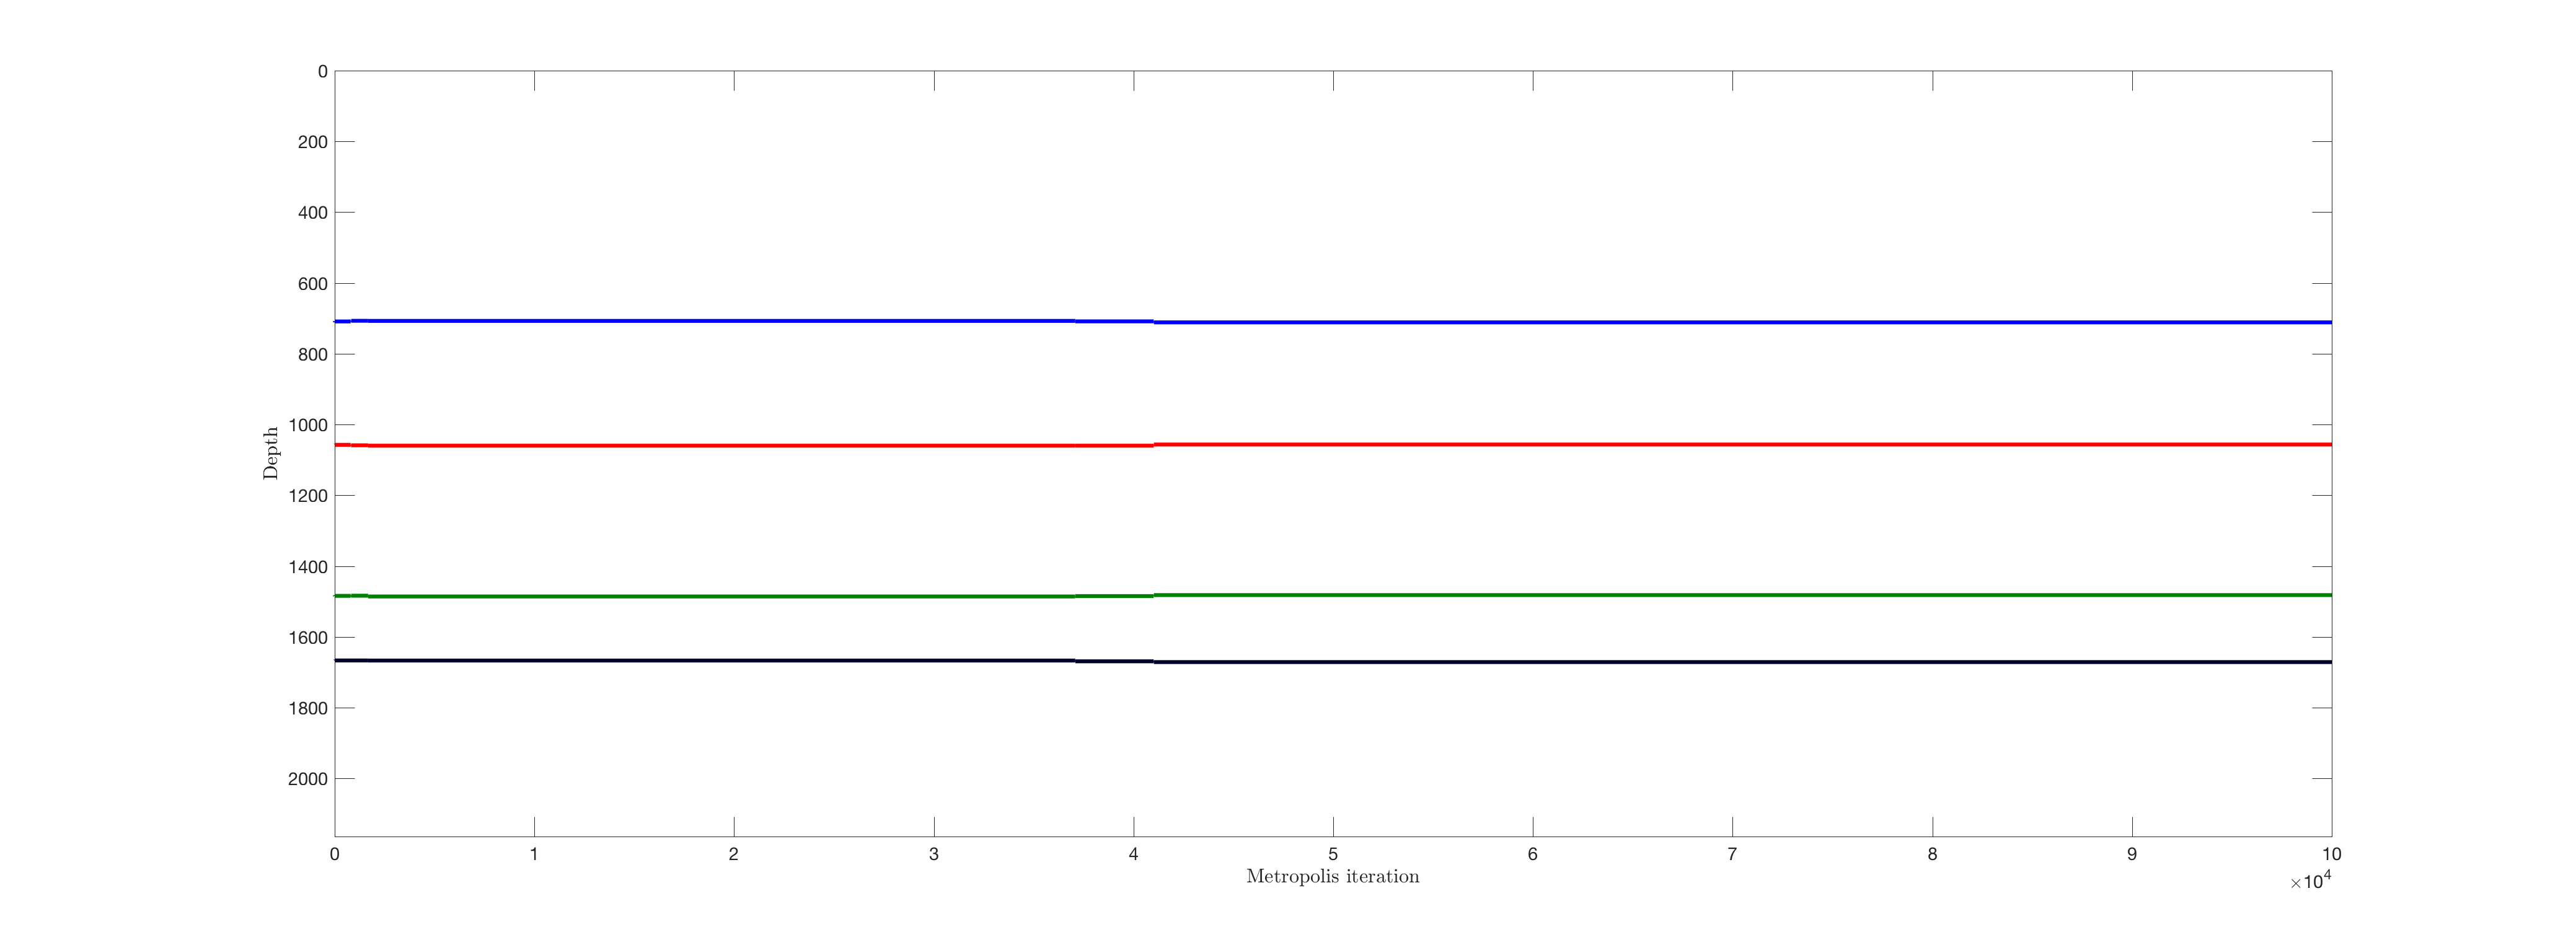
\includegraphics[scale=0.3]{../analysis/figures/convergence3}
%\captionsetup{width=.9\textwidth}
\caption[]{Reflector depth values at each accepted metropolis iteration.}
%\end{center}
\label{fig:depthconvergence}
\end{figure*}



% \section{Firn Correction}

% \begin{figure*}[h]
% %\begin{center}
% \centering
% 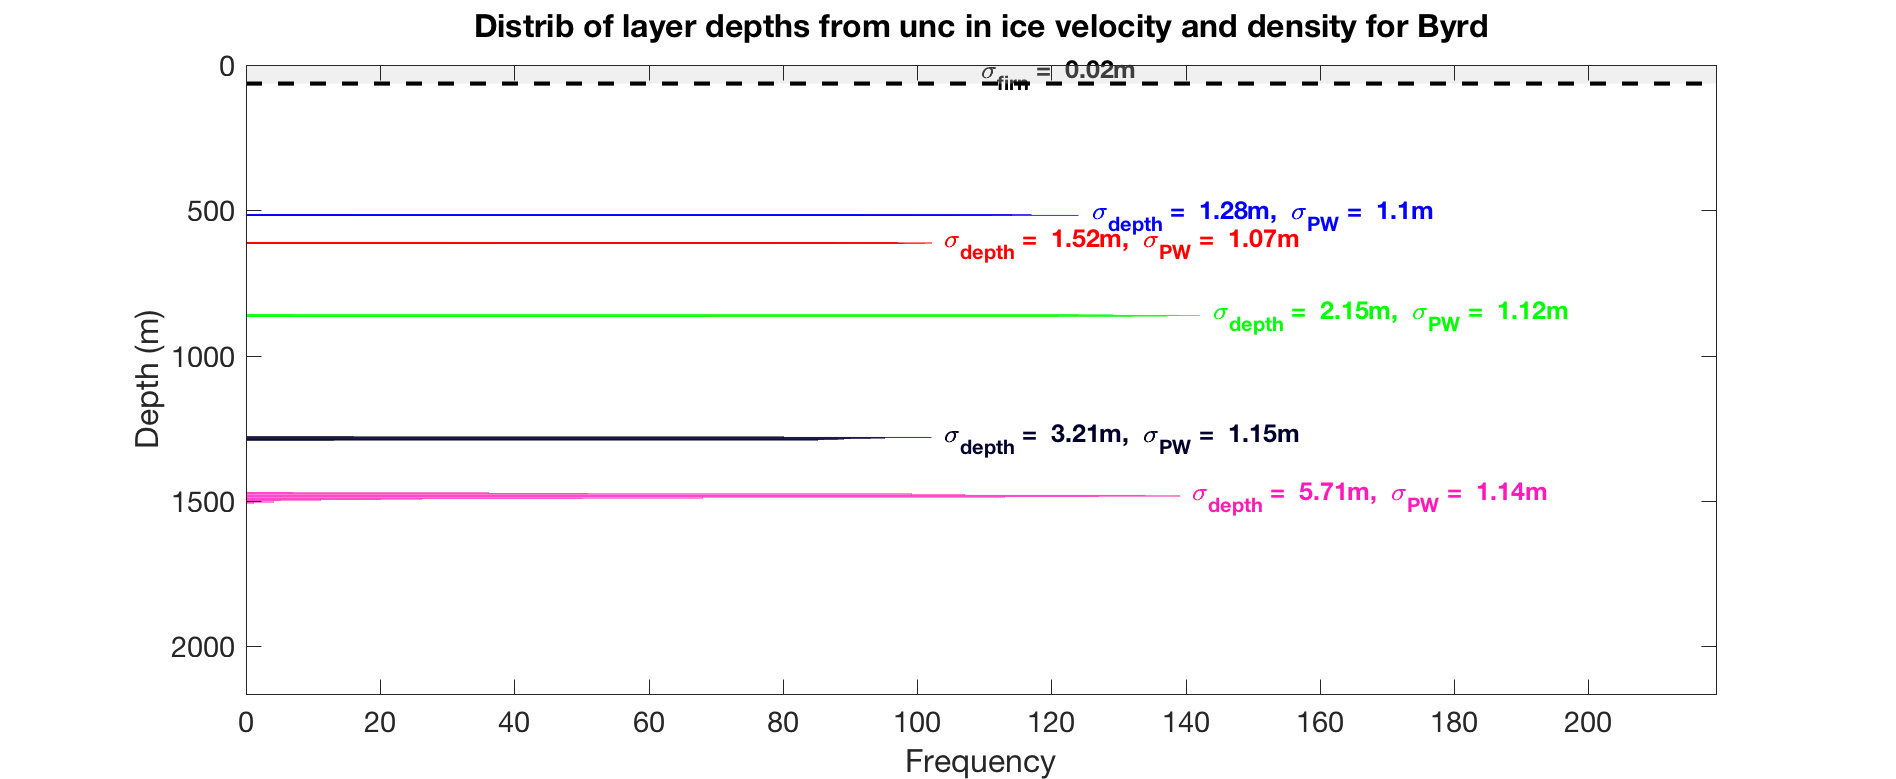
\includegraphics[scale=0.5]{figures/firncorrection}
% %\captionsetup{width=.9\textwidth}
% \caption[]{}
% %\end{center}
% \label{fig:firncorrection}
% \end{figure*}









\section{Regularization}\label{sec:regularization}
\counterwithin{figure}{section} %reset figure numbering

Sampling accumulation rate parameters along the depth profile is inefficient and problematic because many proposed solutions are unrealistically variable. We expect the mean accumulation rate over time (and therefore depth) changes slowly and continuously. To improve our accumulation rate solutions, we regularize the likelihood of reflector age. A regularization parameter is added to the age cost term which punishes proposed accumulation rate profiles which are highly variable relative to a solution computed with no regularization and smoothed over a moving 600-m depth window. This window size is chosen because it is the smallest interval over which the data can be smoothed given the 200-m bin size of the accumulation rate parameters. 

The regularization term, $r$ is the ratio of the variance of a proposed set of accumulation rates to the variance of the smoothed, non-regularized accumulation rate profile. Values of the regularization term for accepted parameter solutions are shown in Figure~\ref{fig:reg}. The regularization is weighted as $r^6$ when included in the calculation of the age cost (Equation~\ref{loglikeage}) to sufficiently reduce variability in the accumulation rate profile. 


\begin{figure*}[ht]
%\begin{center}
\centering
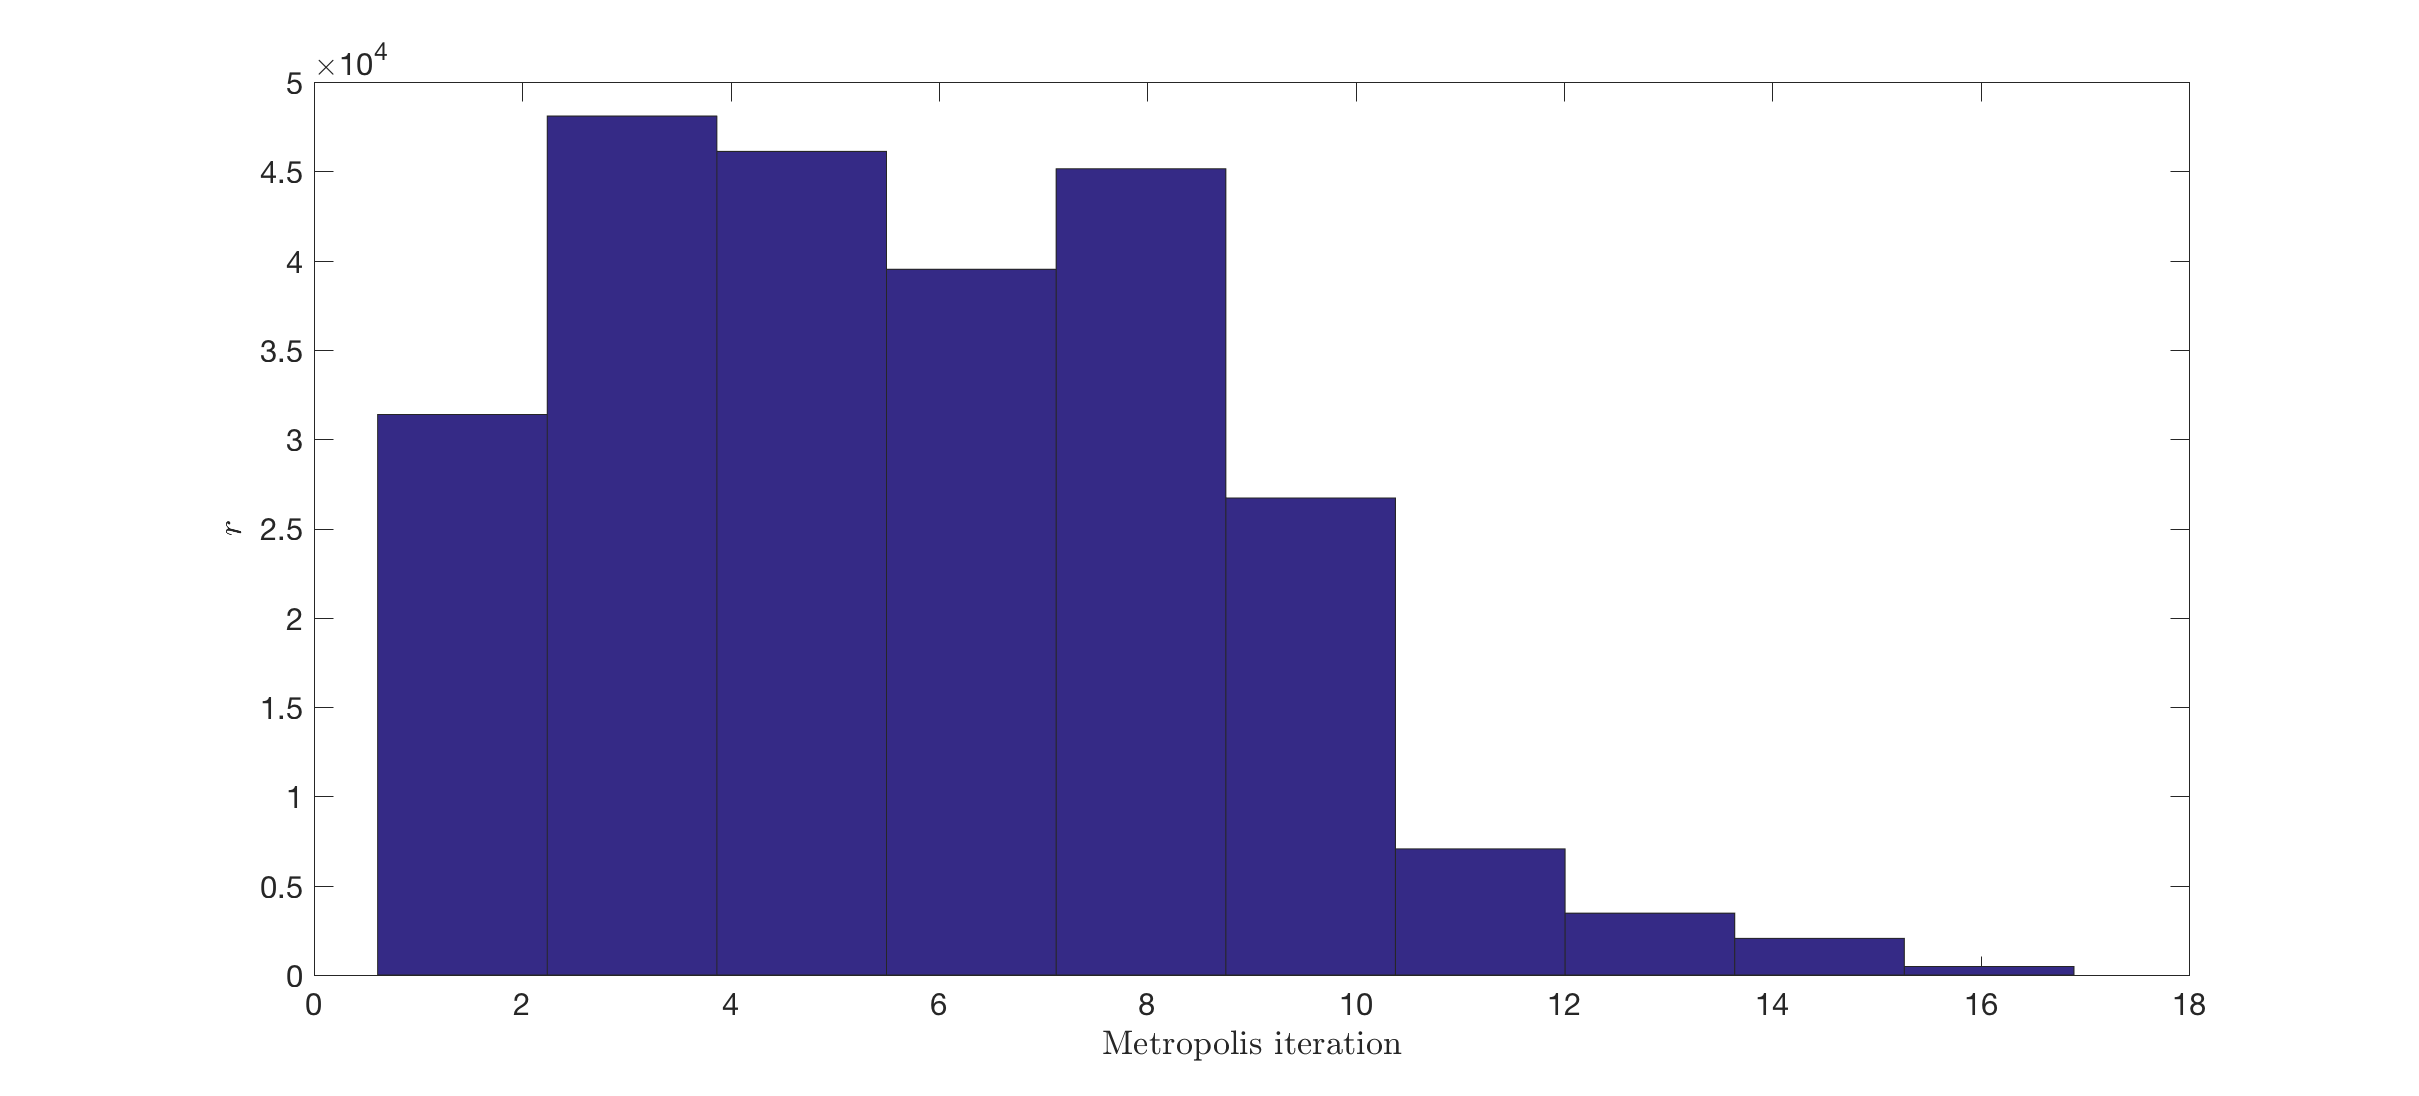
\includegraphics[scale=0.3]{../analysis/figures/regularization}
%\captionsetup{width=.9\textwidth}
\caption[]{Values of the regularization parameter at each accepted metropolis iteration.}
%\end{center}
\label{fig:reg}
\end{figure*}